\section{Auswertung}
\label{sec:auswertung}
In diesem Kapitel sollen die aufgenommenen Messwerte ausgewertet und interpretiert werden.

\subsection{Kennlinien der Hochvakuumdiode}
\label{sec:kennlinien}
In \autoref{fig:schar} sind die Kennlinien der benutzten Hochvakuumdiode bei 5 verschiedenen 
Heizströmen $I_H$ zu sehen, von diesen lassen sich für die in \autoref{tab:stroeme} dargestellten
Sättigungsströme $I_{s}$ ablesen.
\begin{figure}
    \centering
    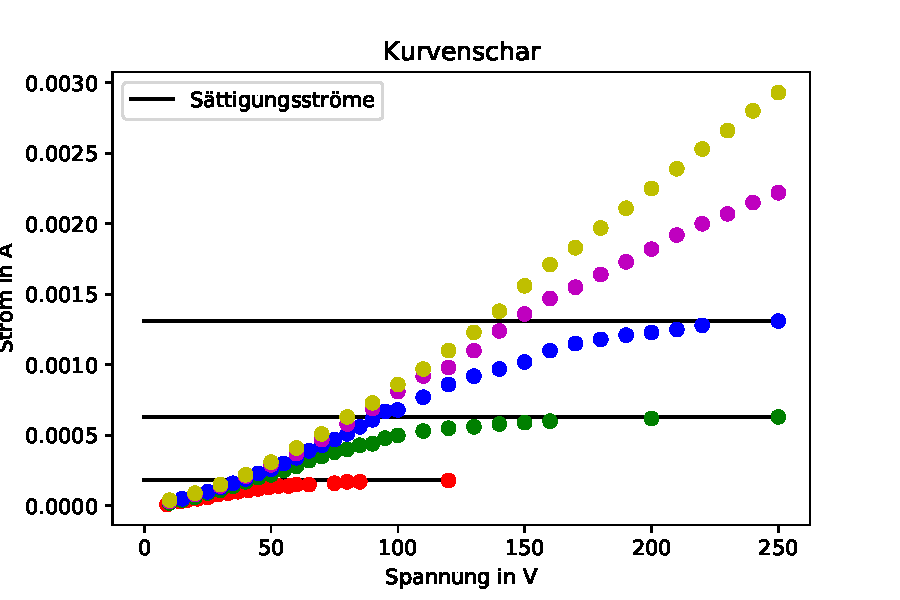
\includegraphics{schar.pdf}
    \caption{Kurvenschar der Ströme in einer Hochvakuumdiode}
    \label{fig:schar}
  \end{figure}
  
  \begin{table}
    \centering
    \caption{Sättigungsströme}
    \label{tab:vergleich}
    \sisetup{table-format=1.2}
    \begin{tabular}{S[table-format=3.2] S S S S  [table-format=3.2]}
      \toprule
      { $I_H$ in A} & {$I_s$ in A}\\
      \midrule
      {$$2.0$$}& {$$ 1.8 \times 10^{-4}$$}\\
      {$$2.2$$}& {$$ 6.3 \times 10^{-4}$$}\\
      {$$2.3$$}& {$$13.1 \times 10^{-4}$$}\\
      {$$2.4$$}& {$$\geq 22.2 \times 10^{-4}$$}\\
      {$$2.5$$}& {$$\geq 29.3 \times 10^{-4}$$}\\
      \bottomrule
    \end{tabular}
  \end{table}
  Für die Heizströme $I_s=2.4\si[]{A}$ und $I_s=2.5\si[]{A}$ lassen sich nur untere Schranken festlegen.
  

  \subsection{Bestimmung des Exponenten der Stom-Spannungs-Beziehung}
  \label{sec:exponent}
  In \autoref{fig:raumladungsgesetz} ist die Kennlinie der Diode bei dem maximal möglichen Heizstrom 
  $I_s=2.5\si[]{A}$ dargestellt und der ungefähre Gültigkeitsbereich des Langmuir-Schottkyschen-Raumladungsgesetzes
  markiert.
  \begin{figure}
    \centering
    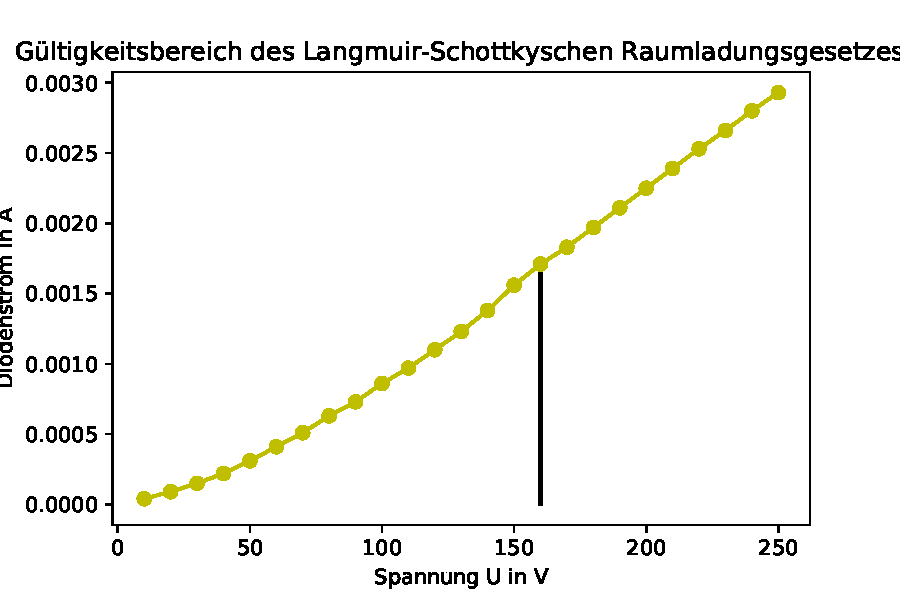
\includegraphics{raumladungsgesetz.pdf}
    \caption{Kurvenschar der Ströme in einer Hochvakuumdiode}
    \label{fig:raumladungsgesetz}
  \end{figure}
  